\section{Comparison of \disappearance fit in disappearance and appearance channels}
\label{app:atmos_channel_comparison}

In this section a comparison of fits of \disappearance using the standard 5 sample fit, the disappearance channel and appearance channel is presented.

Each fit is produced using the standard fit methodology for this analysis, including smearing of the contour in the \dmsq dimension, but the disappearance fit includes the contribution to the $\chi^2$ statistic from only the FHC $\mu$-like and RHC $\mu$-like samples, while the appearance fit includes only the FHC $e$-like, RHC $e$-like and FHC \nueCConepi-like samples.

\begin{figure*}[htb]
	\center
	\begin{subfigure}[b]{0.45\textwidth}
		\center
		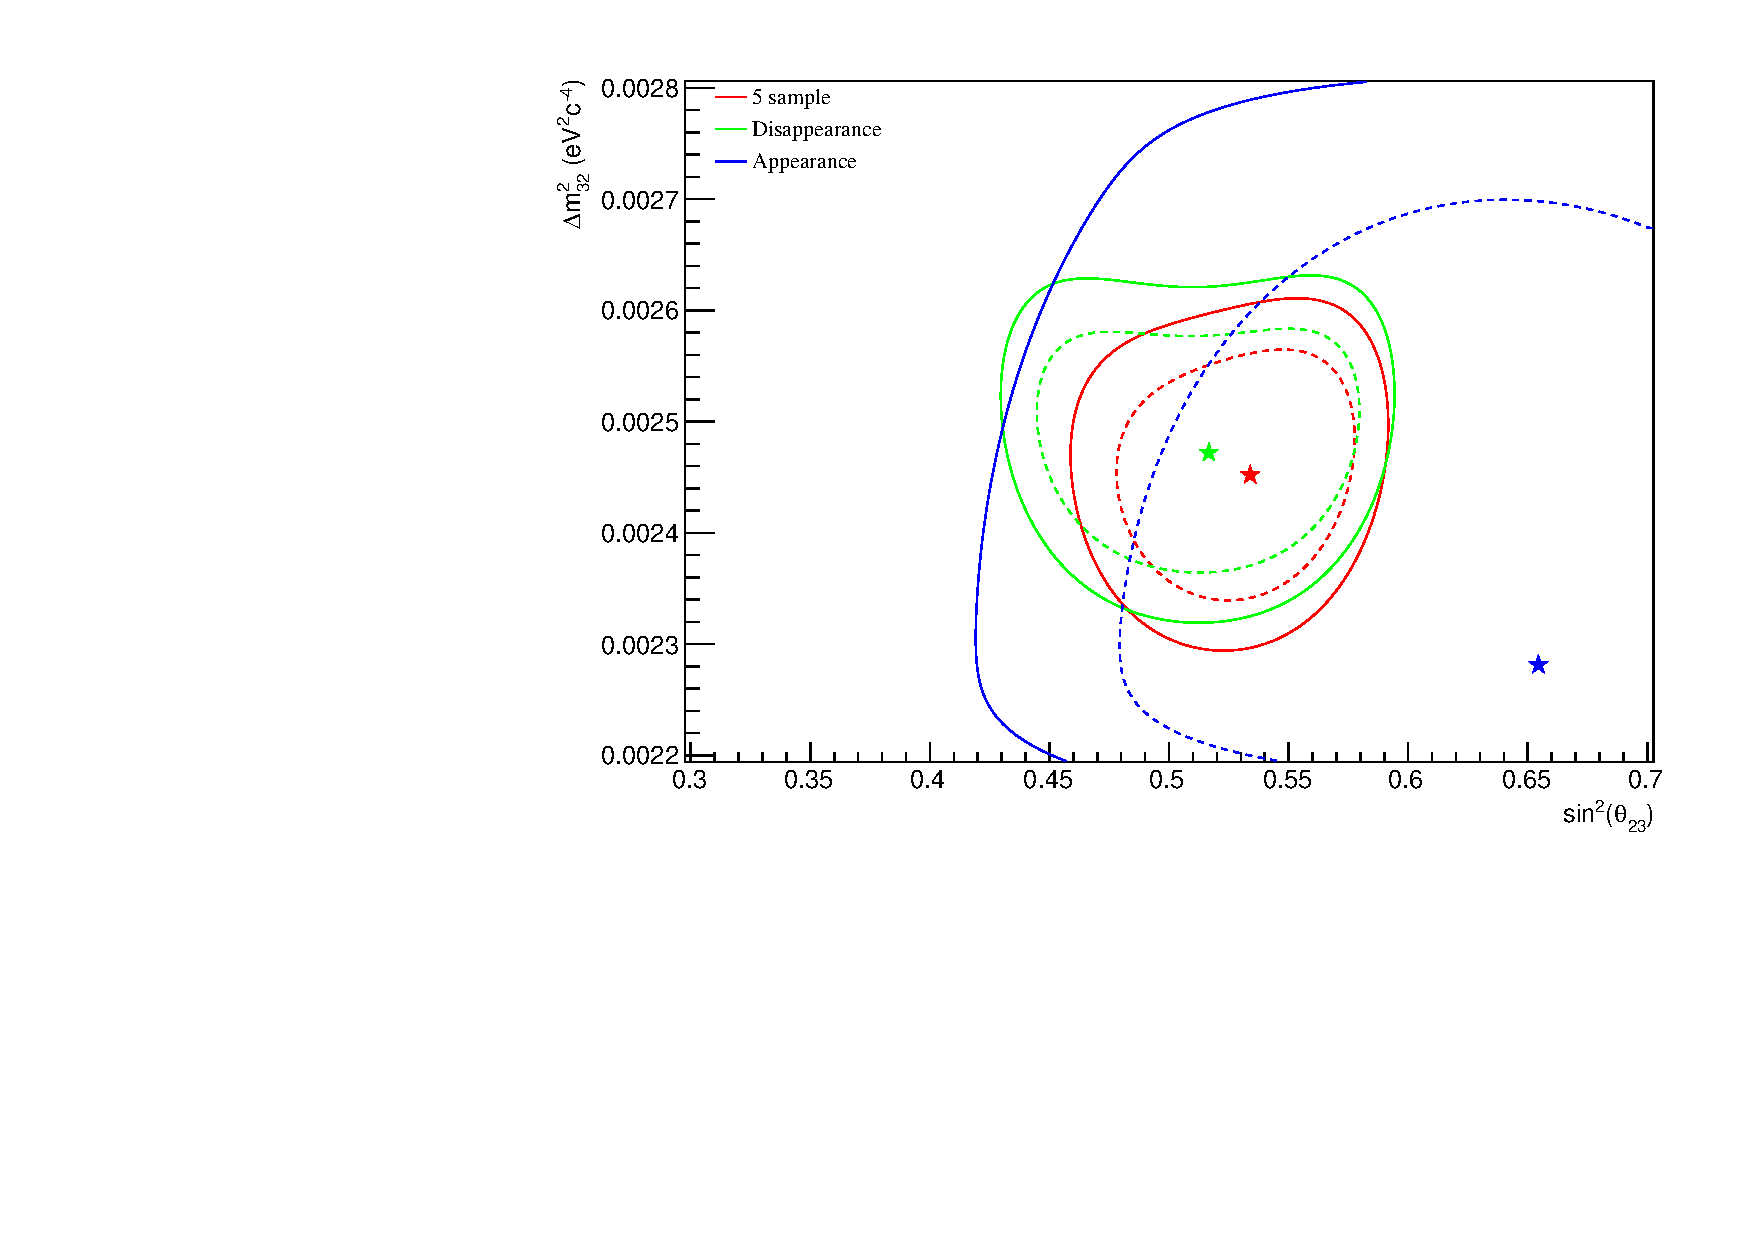
\includegraphics[width=\textwidth]{images/atmos/atmos_nh}
		\caption{Normal}
	\end{subfigure}
	\begin{subfigure}[b]{0.45\textwidth}
		\center
		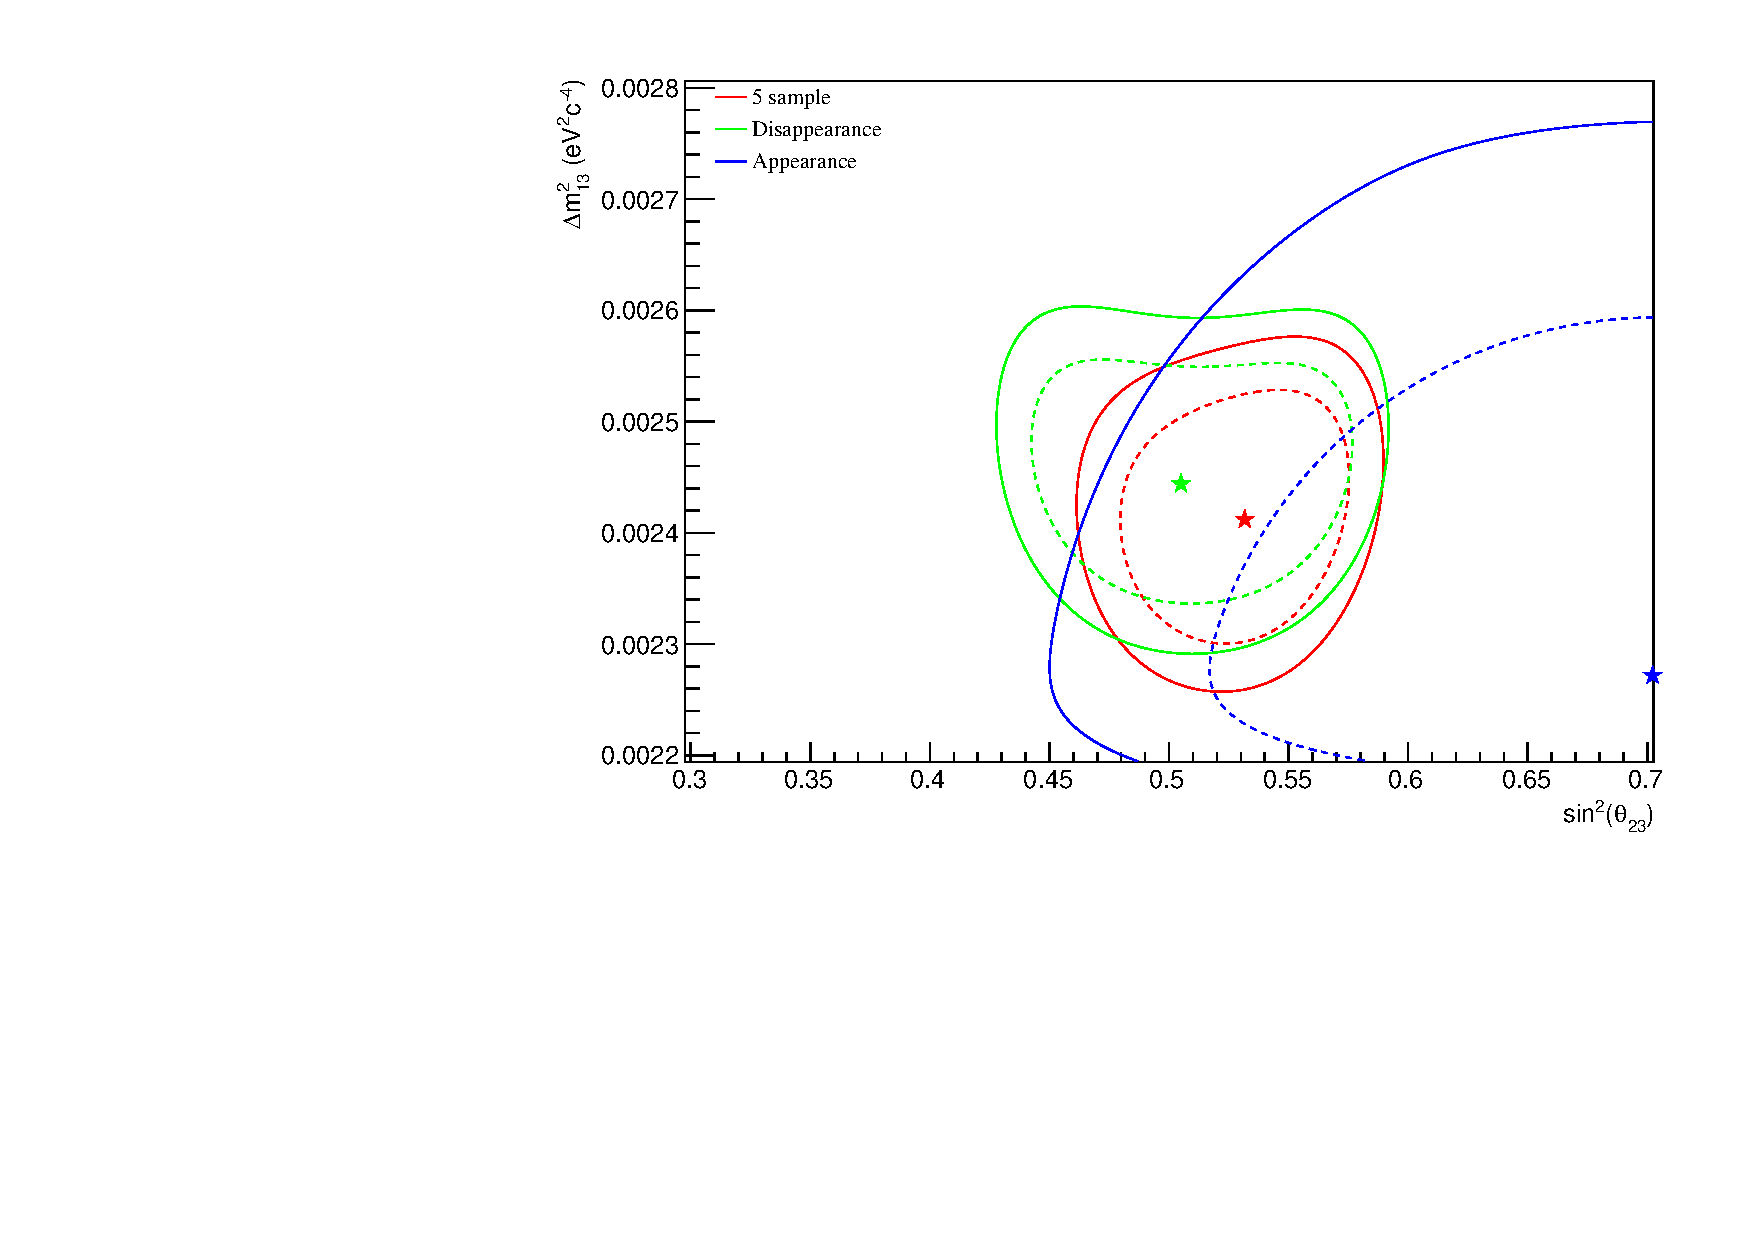
\includegraphics[width=\textwidth]{images/atmos/atmos_ih}
		\caption{Inverted}
	\end{subfigure}
	\caption {
		Fits of \disappearance using all 5 samples, the disappearance channel and the appearance channel.
	}
	\label{fig:atmos_channel_comp}
\end{figure*}

\Cref{fig:atmos_channel_comp} shows that for normal ordering, the three fits are consistent with each other at $68\%$ CL, while for inverted ordering the 5 sample fit and disappearance channel fit have best fit points that fall just outside of the $68\%$ CL for the appearance channel fit. That the appearance channel pulls the best fit to higher values of \ssqthtwothree seems reasonable, given that increasing $\nu_e$ ($\bar{\nu}_e$) event rates are expected for increasing values of \ssqthtwothree in the upper octant (see \cref{fig:bievent}). The behaviour of the best fit with respect to \dmsq is also reasonable; while increasing values of \dmsq would also be expected to produce greater $\nu_e$ ($\bar{\nu}_e$) event rates, the effect size is more modest and at high values of \ssqthtwothree can act to produce better agreement with observation on a rate-only basis. For example, taking $\sin^2\theta_{23} = 0.65$, with other oscillation parameters at best-fit produces a total $\nu_e$ event rate of $\sim91$ compared to $\sim81$ at the best-fit, while taking $\sin^2\theta_{23} = 0.65$ and $\Delta{}m^2_{32} = 2.3\times{}10^{-3}\text{ eV}^2 \text{ c}^{-4}$ reduces the expected event rate to $\sim 90$, consistent with the observed rate.

\clearpage